%%
% Copyright (c) 2017 - 2020, Pascal Wagler;
% Copyright (c) 2014 - 2020, John MacFarlane
%
% All rights reserved.
%
% Redistribution and use in source and binary forms, with or without
% modification, are permitted provided that the following conditions
% are met:
%
% - Redistributions of source code must retain the above copyright
% notice, this list of conditions and the following disclaimer.
%
% - Redistributions in binary form must reproduce the above copyright
% notice, this list of conditions and the following disclaimer in the
% documentation and/or other materials provided with the distribution.
%
% - Neither the name of John MacFarlane nor the names of other
% contributors may be used to endorse or promote products derived
% from this software without specific prior written permission.
%
% THIS SOFTWARE IS PROVIDED BY THE COPYRIGHT HOLDERS AND CONTRIBUTORS
% "AS IS" AND ANY EXPRESS OR IMPLIED WARRANTIES, INCLUDING, BUT NOT
% LIMITED TO, THE IMPLIED WARRANTIES OF MERCHANTABILITY AND FITNESS
% FOR A PARTICULAR PURPOSE ARE DISCLAIMED. IN NO EVENT SHALL THE
% COPYRIGHT OWNER OR CONTRIBUTORS BE LIABLE FOR ANY DIRECT, INDIRECT,
% INCIDENTAL, SPECIAL, EXEMPLARY, OR CONSEQUENTIAL DAMAGES (INCLUDING,
% BUT NOT LIMITED TO, PROCUREMENT OF SUBSTITUTE GOODS OR SERVICES;
% LOSS OF USE, DATA, OR PROFITS; OR BUSINESS INTERRUPTION) HOWEVER
% CAUSED AND ON ANY THEORY OF LIABILITY, WHETHER IN CONTRACT, STRICT
% LIABILITY, OR TORT (INCLUDING NEGLIGENCE OR OTHERWISE) ARISING IN
% ANY WAY OUT OF THE USE OF THIS SOFTWARE, EVEN IF ADVISED OF THE
% POSSIBILITY OF SUCH DAMAGE.
%%

%%
% This is the Eisvogel pandoc LaTeX template.
%
% For usage information and examples visit the official GitHub page:
% https://github.com/Wandmalfarbe/pandoc-latex-template
%%


% @modified: Chuwen <chuwzhang@gmail.com>
% Options for packages loaded elsewhere
\PassOptionsToPackage{unicode}{hyperref}
\PassOptionsToPackage{hyphens}{url}
\PassOptionsToPackage{dvipsnames,svgnames*,x11names*,table}{xcolor}
%
\documentclass[
  a4paper,
,tablecaptionabove
]{scrartcl}
\usepackage{lmodern}
\usepackage{setspace}
\setstretch{1.2}
\usepackage{amssymb,amsmath}
\numberwithin{equation}{section}
\usepackage{ifxetex,ifluatex}
\ifnum 0\ifxetex 1\fi\ifluatex 1\fi=0 % if pdftex
  \usepackage[T1]{fontenc}
  \usepackage[utf8]{inputenc}
  \usepackage{textcomp} % provide euro and other symbols
\else % if luatex or xetex
  \usepackage{unicode-math}
  \defaultfontfeatures{Scale=MatchLowercase}
  \defaultfontfeatures[\rmfamily]{Ligatures=TeX,Scale=1}
\fi
% Use upquote if available, for straight quotes in verbatim environments
\IfFileExists{upquote.sty}{\usepackage{upquote}}{}
\IfFileExists{microtype.sty}{% use microtype if available
  \usepackage[]{microtype}
  \UseMicrotypeSet[protrusion]{basicmath} % disable protrusion for tt fonts
}{}
\makeatletter
\@ifundefined{KOMAClassName}{% if non-KOMA class
  \IfFileExists{parskip.sty}{%
    \usepackage{parskip}
  }{% else
    \setlength{\parindent}{0pt}
    \setlength{\parskip}{6pt plus 2pt minus 1pt}}
}{% if KOMA class
  \KOMAoptions{parskip=half}}
\makeatother
\usepackage{xcolor}
\definecolor{default-linkcolor}{HTML}{A50000}
\definecolor{default-filecolor}{HTML}{A50000}
\definecolor{default-citecolor}{HTML}{4077C0}
\definecolor{default-urlcolor}{HTML}{4077C0}
\IfFileExists{xurl.sty}{\usepackage{xurl}}{} % add URL line breaks if available
\IfFileExists{bookmark.sty}{\usepackage{bookmark}}{\usepackage{hyperref}}
\hypersetup{
  pdfauthor={Chuwen},
  hidelinks,
  breaklinks=true,
  pdfcreator={LaTeX via pandoc with the Eisvogel template}}
\urlstyle{same} % disable monospaced font for URLs
\usepackage[margin=2.5cm,includehead=true,includefoot=true,centering,]{geometry}
% add backlinks to footnote references, cf. https://tex.stackexchange.com/questions/302266/make-footnote-clickable-both-ways
\usepackage{footnotebackref}
\usepackage{graphicx,grffile}
\makeatletter
\def\maxwidth{\ifdim\Gin@nat@width>\linewidth\linewidth\else\Gin@nat@width\fi}
\def\maxheight{\ifdim\Gin@nat@height>\textheight\textheight\else\Gin@nat@height\fi}
\makeatother
% Scale images if necessary, so that they will not overflow the page
% margins by default, and it is still possible to overwrite the defaults
% using explicit options in \includegraphics[width, height, ...]{}
\setkeys{Gin}{width=\maxwidth,height=\maxheight,keepaspectratio}
\setlength{\emergencystretch}{3em}  % prevent overfull lines
\providecommand{\tightlist}{%
  \setlength{\itemsep}{0pt}\setlength{\parskip}{0pt}}
\setcounter{secnumdepth}{3}

% Make use of float-package and set default placement for figures to H.
% The option H means 'PUT IT HERE' (as  opposed to the standard h option which means 'You may put it here if you like').
\usepackage{float}
\floatplacement{figure}{H}
\usepackage{amsthm}
\usepackage[ruled,vlined]{algorithm2e}
\newtheorem{theorem}{Theorem}[section]
\newtheorem{corollary}{Corollary}[theorem]
\newtheorem{lemma}[theorem]{Lemma}
\newtheorem{prop}{Proposition}

\usepackage[UTF8, heading=true]{ctex}
\usepackage{svg}
\svgpath{fig}
\usepackage{booktabs}
\definecolor{tufeijilk}{RGB}{68,87,151}
\hypersetup{colorlinks=true,linkcolor=tufeijilk,urlcolor=cyan}
\newlength{\cslhangindent}
\setlength{\cslhangindent}{1.5em}
\newenvironment{cslreferences}%
  {}%
  {\par}

\author{Chuwen}
\date{\today}



%%
%% added
%%

%
% language specification
%
% If no language is specified, use English as the default main document language.
%

\ifnum 0\ifxetex 1\fi\ifluatex 1\fi=0 % if pdftex
  \usepackage[shorthands=off,main=english]{babel}
\else
  % @update, do not use sfdefault,
  % @chuwen, 20200711
  %   % % Workaround for bug in Polyglossia that breaks `\familydefault` when `\setmainlanguage` is used.
  % % See https://github.com/Wandmalfarbe/pandoc-latex-template/issues/8
  % % See https://github.com/reutenauer/polyglossia/issues/186
  % % See https://github.com/reutenauer/polyglossia/issues/127
  % \renewcommand*\familydefault{\sfdefault}
  %   % load polyglossia as late as possible as it *could* call bidi if RTL lang (e.g. Hebrew or Arabic)
  \usepackage{polyglossia}
  \setmainlanguage[]{english}
\fi



%
% for the background color of the title page
%

%
% break urls
%
\PassOptionsToPackage{hyphens}{url}

%
% When using babel or polyglossia with biblatex, loading csquotes is recommended
% to ensure that quoted texts are typeset according to the rules of your main language.
%
\usepackage{csquotes}

%
% captions
%
\definecolor{caption-color}{HTML}{777777}
\usepackage[font={stretch=1.2}, textfont={color=caption-color}, position=top, skip=4mm, labelfont=bf, singlelinecheck=false, justification=raggedright]{caption}
\setcapindent{0em}

%
% blockquote
%
\definecolor{blockquote-border}{RGB}{221,221,221}
\definecolor{blockquote-text}{RGB}{119,119,119}
\usepackage{mdframed}
\newmdenv[rightline=false,bottomline=false,topline=false,linewidth=3pt,linecolor=blockquote-border,skipabove=\parskip]{customblockquote}
\renewenvironment{quote}{\begin{customblockquote}\list{}{\rightmargin=0em\leftmargin=0em}%
\item\relax\color{blockquote-text}\ignorespaces}{\unskip\unskip\endlist\end{customblockquote}}

%
% heading color
%
\definecolor{heading-color}{RGB}{40,40,40}
\addtokomafont{section}{\color{heading-color}}
% When using the classes report, scrreprt, book,
% scrbook or memoir, uncomment the following line.
%\addtokomafont{chapter}{\color{heading-color}}

%
% variables for title and author
%
\usepackage{titling}
\title{}
\author{Chuwen}

%
% tables
%

%
% remove paragraph indention
%
\setlength{\parindent}{0pt}
\setlength{\parskip}{6pt plus 2pt minus 1pt}
\setlength{\emergencystretch}{3em}  % prevent overfull lines

%
%
% Listings
%
%


%
% header and footer
%
\usepackage{fancyhdr}

\fancypagestyle{eisvogel-header-footer}{
  \fancyhead{}
  \fancyfoot{}
  \lhead[\today]{}
  \chead[]{}
  \rhead[]{\today}
  \lfoot[\thepage]{Chuwen}
  \cfoot[]{}
  \rfoot[Chuwen]{\thepage}
  \renewcommand{\headrulewidth}{0.4pt}
  \renewcommand{\footrulewidth}{0.4pt}
}
\pagestyle{eisvogel-header-footer}

%%
%% end added
%%

\begin{document}

%%
%% begin titlepage
%%

%%
%% end titlepage
%%

{
\setcounter{tocdepth}{3}
\tableofcontents
}
\hypertarget{lagrangian-relaxation}{%
  \section{Lagrangian relaxation}\label{lagrangian-relaxation}}

Consider the following newsvendor-like problem

\[\begin{aligned}
                  & \min f(\delta, \epsilon)                                                                       \\
    \mathbf{s.t.} &                                                                                                \\
                  & y + \delta - \epsilon = b                                                                      \\
                  & y \in \Omega_y \subseteq \mathbb{R}^n, \delta \in \mathbb{R}^n_+ , \epsilon \in \mathbb{R}^n_+
  \end{aligned}\]

where \(f\) is a convex function of \(\delta, \epsilon\). The
right-hand-side on the binding constraints is in the positive orthant:
\(b \in \mathbb R_+^n.\) This problem widely appears in applications of
device maintenance, inventory management, and so on. In the basic
settings, let \(y\) be the ordering quantity quantities in a multi-item
newsvendor problem, one minimizes the total expected cost:

\[\min_{y \in \mathbb R_+} \mathbf E\left(h\cdot e^\mathsf{T} \max\{y - b,  0\} + p \cdot e^\mathsf{T} \max\{b - y,  0\}\right)\]

It is easy to verify its equivalence to the problem above.

Let \(\lambda\in\mathbb{R}^n\) be the Lagrangian multiplier, the dual
function is:

\[\begin{aligned}
    \phi(\lambda) = & \min_{\delta, \epsilon} f(\delta, \epsilon) + \lambda^\mathsf{T}\delta - \lambda^\mathsf{T} \epsilon+ \min_y \lambda^\mathsf{T} y - \lambda^\mathsf{T} b \\
    \mathbf{s.t.}   &                                                                                                                                                          \\
                    & y \in \Omega_y                                                                                                                                           \\
                    & \delta \in \mathbb{R}^n_+ , \epsilon \in \mathbb{R}^n_+
  \end{aligned}\]

We assume the resulting two subproblems for \(\delta, \epsilon\) and
\(y\) are easy.

\hypertarget{affine-case}{%
  \subsection{Affine case}\label{affine-case}}

\textbf{The case for repair problem}

Let \(f=p^\mathsf{T}\delta + h^\mathsf{T} \epsilon\), we have

\[\phi(\lambda) = \min_{\delta, \epsilon} (p+ \lambda)^\mathsf{T}\delta + (h - \lambda)^\mathsf{T} \epsilon+ \min_y \lambda^\mathsf{T} y - \lambda^\mathsf{T} b\]

Then \(\phi\) is unbounded unless \(\lambda \in \Lambda\) where
\(\Lambda = \{\lambda: \lambda \in [-p, h]\}\), in which case

\[\phi(\lambda) = \min_{y\in \Omega_y} \lambda^\mathsf{T} y - \lambda^\mathsf{T} b,\; \lambda\in \Lambda\]

and \(\delta^\star, \epsilon^\star = 0\) are corresponding optimizers
for any \(\lambda \in \Lambda\)

\hypertarget{conditions-for-strong-duality}{%
  \subsection{Conditions for strong
    duality}\label{conditions-for-strong-duality}}

It's well known that strong duality does not hold in general. We review
some of the cases here. The Lagrangian duality theory can be found in
any standard text.

\begin{enumerate}
  \def\labelenumi{(\alph{enumi})}
  \tightlist
  \item
        if \(\Omega_y\) is convex then the strong duality holds \ldots,
        i.e.~\(\phi^\star = f^\star\)
\end{enumerate}

\ldots{} add justifications here (slater, \ldots)

A more interesting result is devoted to mixed integer problems.
\textbf{(Review Here)}.

\begin{enumerate}
  \def\labelenumi{(\alph{enumi})}
  \setcounter{enumi}{1}
  \tightlist
  \item
        if
        \(\Omega_y = \{y \in \mathbb R^n: y \in \Omega, y\in \mathbb Z^n\}\).
        Then we have the following relation for dual function,
\end{enumerate}

\[ \phi^\star = \min_{\delta, \epsilon} f(\delta, \epsilon)\quad \textbf{ s.t. }  y + \delta - \epsilon = b,\; y \in \textrm{conv}(\Omega_y)\]

We conclude the strong duality holds since
\(Y = \{(y, \delta, \epsilon): y + \delta - \epsilon = b,\; y \in \textsf{conv}(\Omega_y)\}\)
is already \emph{a perfect formulation} in the sense that
\(Y = \textsf{conv}(Y)\)

\textbf{add a proposition to show this or add more conditions to
  justify}


\hypertarget{subgradient-method}{%
  \section{Subgradient method}\label{subgradient-method}}

To solve the reduced problem, we consider a variant of subgradient
method:

\[\lambda^{k+1} = \mathbf{P}(\hat \lambda^{k} + s^{k}\bar g^{k})\]

where \(\mathbf P\) is the projection onto dual space
\(\{\lambda: \lambda \in [-c, d]\}\). \(\hat \lambda^k\) is the
multiplier associated with the best dual bound:

\[\hat \phi^k = \max_{t=1, ..., k} \phi(\lambda^t)\]

\(\bar g^k\) is the update direction for current iteration and \(s^{k}\)
is the step size using target-based rules:

\[s^{k} = \frac{\phi^\star - \phi(\lambda^k)}{||\bar g^{k}||^2}\]

Note the direction \(\bar g^k\) computed by \(\bar g^k = \bar y^k - d\), where \(\bar y^k\) is the convex combination of previous iterations
\(y^1, ..., y^k\) such that \(y^k\) solves \(\phi^k = \phi(\lambda^k)\).

\[\bar y^k = (1-\alpha)\cdot\bar y^{k-1} + \alpha \cdot y^k \]

For simplicity we let \(g^k= y^k - d\), then \(g^k\) is a subgradient of
\(\phi\) at \(\lambda^k: g^k \in \partial \phi^k\), we can write the direction as the combination of the subgradient and
previous directions:

\[\bar g^k = (1-\alpha) \bar g^{k-1} + \alpha\cdot g^k\]

The target based rule are well-known as the Polyak rule \cite{polyak_general_1967}. The idea of using previous searching directions is introduced to accelerate the subgradient method and provide a better stopping criterion,
see \cite{camerini1975improving}, \cite{brannlund1995generalized}, \cite{barahona_volume_2000}. Brannlund \cite{brannlund1995generalized} showed that
with convex combinations the optimal choice of stepsize is equivalent to the Camerini-Fratta-Maffioli modification, it also provides an analysis on its linear convergence rate.
Barahona and Anbil \cite{barahona_volume_2000} uses a slight different modification to approximate the primal feasible solutions in the dual searching process.


It is obvious to see the solutions during dual optimization
\((y, \epsilon, \delta) = (y^k, 0, 0)\) are feasible if and only if we
can find \(y^k = d\), which in general will not hold. This motivates the
following heuristic.

\begin{algorithm}[H]
  \SetAlgoLined
  \[\begin{aligned}
      \epsilon^k = \max\{y^k - d, 0\} \\
      \delta^k = \max\{d - y^k, 0\}
    \end{aligned}\]
  \caption{Recovery Heuristic}
\end{algorithm}

Let the primal objective value be \(z^k\). We apply same averaging scheme to produce \((\bar \delta^k, \bar \epsilon^k)\), and record the
corresponding primal objective value as \(\bar z^k\) such that \(\bar z^k = f(\bar \delta^k, \bar \epsilon^k)\).
The dual subgradient algorithm can be summarized as follows.

\begin{algorithm}[H]
  \SetAlgoLined
  ...
  \While{...}{
    ...
  }
  \caption{The Subgradient Algorithm (Volume)}
\end{algorithm}

\textbf{Computational results}
The typical convergence of \(\bar z^k\) and \(\hat \phi^k\) computed
from the repair model can be shown: (green - \(z^k\), orange -
\(\bar z^k\), blue - \(\hat \phi^k\))

% 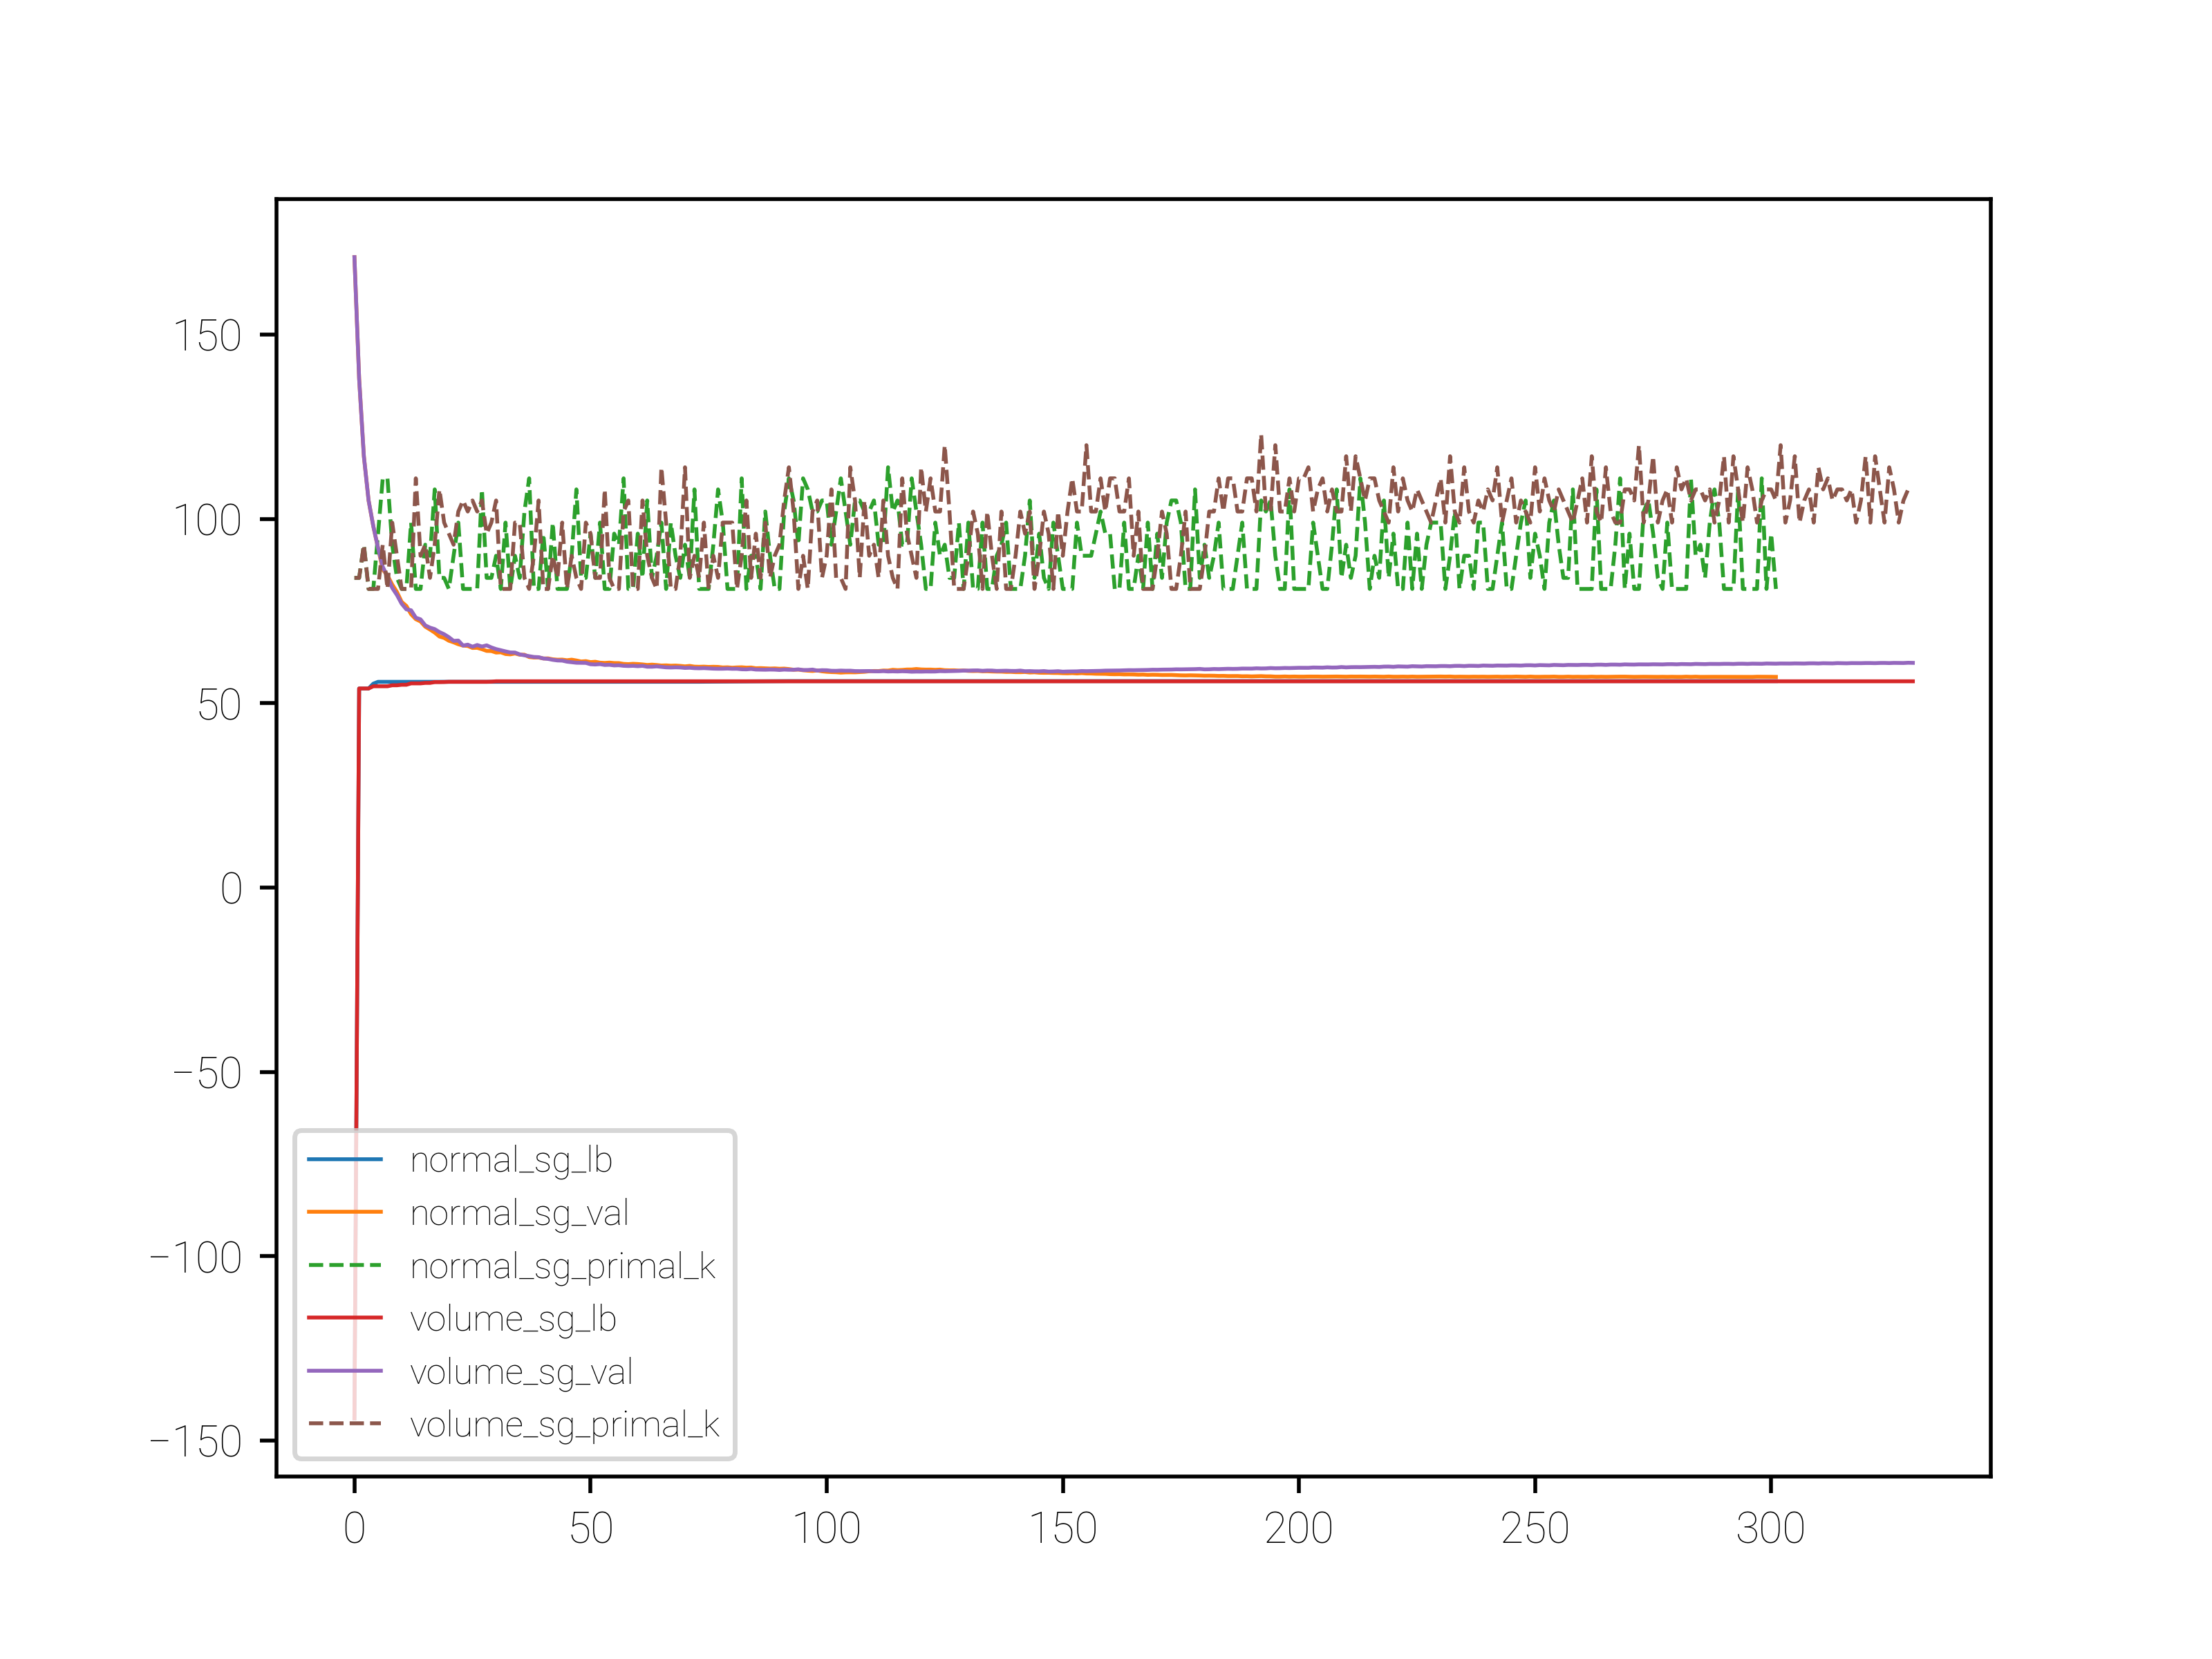
\includegraphics{fig/conv_0_10_20.png}

and test on a group of examples (the repair model)


\hypertarget{subgradient-method}{%
  \section{Convergence}\label{Convergence}}

\textbf{(We wish to show the convergence):} \(|\bar z^k -\hat \phi^k|\)



Nedi´c

We first review several properties for the subgradient method outlined in \ref{prop1}.
We adopt some of the results in Camerini-Fratta-Maffioli modification \cite{camerini1975improving}
and the analysis of using convex combination of previous iterations in \cite{brannlund1995generalized}

\begin{lemma} \label{prop1}
  Properties for subgradient method\\
  \begin{enumerate}
    \item
          \begin{equation}\label{eq:simplified_dual_conv}
            2 \langle d^k, \lambda^\star - \hat \lambda^k \rangle \ge \rho (\phi^\star - \hat \phi^k) =  s^k ||d^k||^2
          \end{equation}
    \item by \eqref{eq:simplified_dual_conv}, hopefully we have:
          \begin{equation}\label{eq:dual_conv}
            ||\hat \lambda^{k+1} - \lambda^\star|| \le ||\hat \lambda^{k} - \lambda^\star||
          \end{equation}
  \end{enumerate}
\end{lemma}

% \begin{proof}
%   1. Can be proved by induction?\\
%   \(k = 1\), \(d^k = g^k\), by convexity we have:
%   \[\langle d^k, \lambda^\star - \lambda^k  \rangle = \langle g^k, \lambda^\star - \lambda^k  \rangle \ge \phi^\star - \phi^k \]
%   Let us assume the relation holds for \(k\), consider iteration \(k+1\). First notice:
%   \begin{equation}\label{eq:min_phi}
%     \langle g^{k+1} ,\hat \lambda^k \rangle \ge \hat \phi^k
%   \end{equation}

%   Since \(\hat\lambda^{k+1}\) takes values in \(\{\hat \lambda^k, \lambda^{k+1}\}\), we prove for each case.

%   (a) \(\hat \lambda^{k+1} = \lambda^{k+1}\), which implies: \(\phi^{k+1} = \hat \phi^{k+1} \ge \hat \phi^k\)
%   \[\begin{aligned}
%       \langle d^{k+1}, \lambda^\star - \lambda^{k+1}\rangle
%        & = \langle \alpha g^{k+1} + (1-\alpha) d^k, \lambda^\star - \lambda^{k+1}\rangle                                                              \\
%        & \ge \alpha (\phi^\star - \phi^{k+1}) + (1-\alpha)\cdot \langle d^k, \lambda^\star - \hat \lambda^k - s^k d^k\rangle                          \\
%        & \stackrel{\eqref{eq:simplified_dual_conv}}{\ge} \alpha (\phi^\star - \phi^{k+1}) + (1-\alpha) ( \frac{1}{2}\rho -1)(\phi^\star - \phi^{k+1}) \\
%        & \ge (\phi^\star - \phi^{k+1})
%     \end{aligned}\]
%   (b) \(\hat \lambda^{k+1} = \hat \lambda^{k}\), and thus: \(\hat \phi^{k+1} = \hat \phi^{k} \ge  \phi^{k+1}\)
%   % \langle, \rangle
%   \[\begin{aligned}
%       \langle d^{k+1}, \lambda^\star - \hat\lambda^k\rangle
%        & = \langle \alpha g^{k+1} + (1-\alpha) d^k, \lambda^\star - \hat\lambda^k\rangle                                                                    \\
%        & \ge (1-\alpha) \cdot (\phi^\star - \hat \phi^k) + \alpha\cdot \langle \lambda^\star - \hat\lambda^k, g^{k+1} \rangle                               \\
%        & = (1-\alpha) \cdot (\phi^\star - \hat \phi^k) + \alpha\cdot \langle \lambda^\star - \lambda^{k+1} + \lambda^{k+1} - \hat\lambda^k, g^{k+1} \rangle \\
%        & \stackrel{\eqref{eq:min_phi}}{\ge} (1-\alpha) \cdot (\phi^\star - \hat \phi^k) + \alpha\cdot(\phi^\star - \phi^{k+1} + \phi^{k+1} - \hat \phi^k)   \\
%        & =\phi^\star - \hat \phi^{k+1}
%     \end{aligned}\]
% \end{proof}

% \begin{proof}
%   2. like 1, and we use \label{eq:simplified_dual_conv}
%   \[
% \begin{aligned}
%   \left\|\lambda^{k+1}-\lambda^{*}\right\|^{2}
%    & \leq\left\|\hat\lambda^{k}+s^{k} d^{k}-\lambda^{*}\right\|^{2}                                                                                                               \\
%    & \leq\left\|\hat \lambda^{k}-\lambda^{*}\right\|^{2} - 2 \langle s^{k}d^{k}, \left(\lambda^{*}-\hat \lambda^{k}\right)\rangle +\left(s^{k}\right)^{2}\left\|d^{k}\right\|^{2} \\
%    & = \left\|\hat \lambda^{k}-\lambda^{*}\right\|^{2} - s^k \left ( 2 \langle d^k, \lambda^{*}-\hat \lambda^{k}\rangle - s^k \|d^k\|^2 \right )
% \end{aligned}\]

%   We have to show:


% \end{proof}
% \[\begin{aligned}
%     \langle\lambda^\star - \lambda^k, g^k\rangle = \langle\lambda^\star - \hat\lambda^k + \hat\lambda^k -\lambda^k, g^k\rangle \\
%     \langle\hat\lambda^k - \lambda^k, g^k\rangle \ge \hat \phi^k - \phi^k \ge 0
%   \end{aligned}\]




\textbf{Proposition 2}.

\begin{enumerate}
  \def\labelenumi{(\alph{enumi})}
  \tightlist
  \item
        For fixed \(y=y^k\), \((\epsilon^k, \delta^k)\) is the optimal
        solution for the restricted primal problem.
\end{enumerate}

\[f(\epsilon^k, \delta^k) \le f(\epsilon, \delta), \quad \forall \delta\ge 0, \epsilon\ge 0, y= y^k\]

\begin{enumerate}
  \def\labelenumi{(\alph{enumi})}
  \setcounter{enumi}{1}
  \tightlist
  \item
        \(\bar z^k \le \bar f(\delta^k, \epsilon^k)\)
\end{enumerate}

\textbf{PF.} By convexity.

\hypertarget{computational-results}{%
  \subsection{Computational results}\label{computational-results}}

\hypertarget{repair-problem}{%
  \subsubsection{Repair problem}\label{repair-problem}}

\hypertarget{general-case}{%
  \subsubsection{General case}\label{general-case}}

\addcontentsline{toc}{section}{References}

\hypertarget{refs}{}
\bibliography{repair}
\bibliographystyle{siam}

\end{document}
